\documentclass[11pt]{article}
\usepackage[utf8]{inputenc}
\usepackage[ngerman]{babel}

\usepackage{amsmath,amsthm,amssymb,amsfonts}

\usepackage{graphicx}
\usepackage{float}
\usepackage{tikz}

\usepackage{fancyhdr} % For headers and footers
\usepackage{geometry}
\usepackage{listings}
\usepackage{hyperref}
\hypersetup{
    linkcolor=blue,     
    urlcolor=cyan,
}

\geometry{
    a4paper, % Change this if you intend to print on a different paper size, such as letter paper.
    left=20mm,
    right=20mm,
    top=30mm,
    bottom=30mm,
}

\newcount\colveccount
\newcommand*\colvec[1]{
        \global\colveccount#1
        \begin{pmatrix}
        \colvecnext
}
\def\colvecnext#1{
        #1
        \global\advance\colveccount-1
        \ifnum\colveccount>0
                \\
                \expandafter\colvecnext
        \else
                \end{pmatrix}
        \fi
}

\title{Statik - Gleichgewichtsbedingungen für Translation und Rotation}
\author{Emil Staikov}
\date{14. Juni 2021}

\begin{document}
\maketitle
Bis jetzt haben wir uns in der Mechanik mit verschiedenen Bewegungen auseinandergesetzt. Oftmals ist es aber auch interessant, Anordnungen zu betrachten, die sich nicht bewegen, also in einem Gleichgewicht sind. Mit solchen Problemen beschäftigt die Statik. 


\section{Gleichgewichtsbedingungen}
Ein System im statischen Gleichgewicht erfüllt einige Bedingungen. 
\subsection{Kräfte und Drehmomente}
Für ein System im Gleichgewicht gilt $\vec{a} = 0$ und $\vec{\alpha} = 0$. Damit gilt nach dem zweiten Newtonschen Axiom für Translation bzw. Rotation 
\begin{equation*}
        \sum \vec{F}_{ext} = m\vec{a} = 0 \quad \quad \sum \vec{M}_{ext} = m\vec{\alpha} = 0
\end{equation*}
Damit schließen wir auf die Komponentengleichungen 
\begin{gather*}
        \sum F_x = 0 \quad \quad \sum F_y = 0 \quad \quad \sum F_z = 0 \\
        \sum M_x = 0 \quad \quad \sum M_y = 0 \quad \quad \sum M_z = 0 
\end{gather*}
Für ein System im Gleichgewicht können wir diese Gleichungen aufstellen und lösen. Dabei summieren sich die Drehmomente um jede beliebige Achse weg, man wählt die Achse meistens so, dass möglichst viele Drehmomente wegfallen. Drehmomente fallen weg, wenn die zugehörigen Kräfte in der Achse selbst ansetzen ($r = 0$), oder senkrecht zum Radius wirken. 
\subsection{Energie (qualitativ)}
Wir unterscheiden, abhängig von der potentiellen Energie des Systems, hauptsächlich zwei Arten von Gleichgewichten. Ein System ist physikalisch gesehen im Gleichgewicht, wenn sich, vereinfacht gesagt, nichts bewegt. \\\\
In einem \textbf{stabilen Gleichgewicht} wird das System nach einer leichten Änderung der Konfiguration weg von dem Gleichgewicht zu der Gleichgewichtskonfiguration zurückkehren. EIn Beispiel dafür ist ein Fadenpendel. Wenn dieses aus der Ruhelage ausgelenkt wird, schwingt es, bis es durch Reibung Energie so viel Energie abgibt, dass es wieder in der Ruhelage landet. Ein System befindet sich in einem stabilen Gleichgewicht, wenn seine potentielle Energie dort lokal minimal ist. \\
In einem \textbf{instabilen Gleichgewicht} wird sich das System nach einer leichten Änderung der Konfiguration weg von dem Gleichgewicht weiter von der Gleichgewichtsposition wegbewegen. EIn Beispiel dafür ist eine Kugel auf einer Hügelspitze, wenn sie leicht angestoßen wird, rollt sie den ganzen Hügel herunter. Im Tal befindet sie sich wiederum in einem stabilen Gleichgewicht. Ein System befindet sich in einem instabilen Gleichgewicht, wenn seine potentielle Energie dort lokal maximal ist. \\\\
Systeme, die in der Statik betrachtet werden, befinden sich meistens in einem stabilen Gleichgewicht. Minima bzw. Maxima der potentiellen Energie zu bestimmen ist jedoch mathematisch relativ anspruchsvoll, dieser Ansatz ist für die IJSO daher weniger relevant. 


\section{Ansatz bei Gleichgewichtsaufgaben}
\textbf{1.:} Zuerst ist die Grenze des Systems zu bestimmen, um klarzustellen, welche Kräfte und Drehmomente extern bzw. intern sind. \\\\
\textbf{2.:} Zeichne ein Diagramm, genannt Freikörperdiagramm, in dem alle Objekte im System, die auf sie wirkenden äußeren Kräfte und ihre zugehörigen Angriffspunkte (im allgemeinen der Schwerpunkt) eingezeichnet sind. Teilweise ist die Wirkungsrichtung von Kräften nicht im Voraus bekannt. In dem Fall nimmt man einfach eine Richtung an, wenn sich diese als falsch herausstellt, wird das errechnete Endergebnis negativ sein. \\\\
\textbf{3.:} Wähle ein Koordinatensystem, anhand dessen die Kräfte in Komponenten zerlegt werden. Es bietet sich an, das Koordinatensystem so zu wählen, dass möglichst viele Kräfte mit den Achsen zusammenfallen. \\\\
\textbf{4.:} Wähle eine Rotationsachse und ein zugehöriges Koordinatensystem (ein Koordinatensystem, in dem die Rotationsachse durch den Ursprung geht), um die externen Drehmomente zu zerlegen. Ein Drehmoment ist positiv, wenn seine Wirkung zu einer Rotation entgegen des Uhrzeigersinns um die Drehachse führt, sonst negativ.  \\\\
\textbf{5.:} Stelle die Komponentengleichungen auf und setze sie gleich null, löse sie dann nach den gesuchten Größen. 

\pagebreak
\section{Beispiele}
\textbf{Aufgabe:} Die Enden einer Platte der Länge $L$ mit uniform verteilter Masse $m = 1.8kg$ liegen auf zwei Waagen. Im Abstand $L/4$ von dem einen Ende der Waage befindet sich der Schwerpunkt eines Blocks der Masse $M = 2.7kg$, der auf der Platte steht. Welche Kräftebeträge wirken jeweils auf die einzelnen Waagen? \\\\
\textbf{Diagramme:}
\begin{figure}[H] 
        \centering
        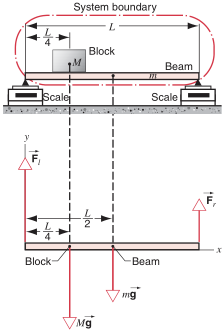
\includegraphics{abb/1-statik-rot-tra/aufgabe-1.png}
        \caption{oben: Schematisches Diagramm des Aufbaus, unten: Freikörperdiagramm (Kräfte und ihre Angriffspunkte, Komponenten nur angedeutet), Abbildung aus HRK Vol. 1}
\end{figure}
\noindent\textbf{Lösung:} Durch die Abbildung oben sind Systemgrenze, Freikörperdiagramm und die $x$-Achse bereits festgesetzt. Als externe Kräfte wirken die Gravitation auf Masseblock und Platte, sowie die Kräfte durch die beiden Waagen. Alle äußeren Kräfte haben einzig Komponenten in $y$-Richtung, daher ergibt sich nur eine Kräftegleichung: 
\begin{equation}
        F_l + F_r - Mg - mg = 0
\end{equation}
$F_l$ und $F_r$ wirken in die gleiche Richtung, $mg$ und $Mg$ genau in die entgegengesetzte. $F_l$ und $F_r$ haben folglich untereinander gleiche Vorzeichen, $mg$ und $Mg$ genauso, zwischen den beiden Paaren unterscheidet sich das Vorzeichen aber. \\
Mit der Kräftegleichung können wir noch nicht die unbekannten $F_l$ und $F_r$ bestimmen. Daher stellen wir noch eine Drehmomentgleichung auf, doch um welchen Punkt? Prinzipiell können wir jeden beliebigen Punkt wählen, von dem aus wir die Abstände zu den verschiedenen Kräften ermitteln können. Wie bereits erwähnt bietet es sich aber besonders an, den Punkt so zu wählen, dass einige der unbekannten Terme wegfallen. In dem Fall bietet sich z.B. der Berührpunkt der linken Waage an. \\
$F_l$ greift direkt an der Achse an, hat also damit Radius null. Das zugehörige Drehmoment ist dann also $M_l = r_lF_l = 0F_l = 0$. Die restlichen zugehörigen Drehmomente ermitteln wir entsprechend: $M_m = -\frac{L}{2}mg$, $M_M = -\frac{L}{4}Mg$ und $M_r = LF_r$. Wir folgen hier der oben beschriebenen Vorzeichenkonvention für Drehmomente. Daraus ergibt sich folgende Drehmomentgleichung, die wir gleich nach $F_r$ auflösen können 
\begin{align}
        0 &= LF_r - \frac{L}{2}mg - \frac{L}{4}Mg \nonumber \\
        \iff LF_r &= \frac{L}{2}mg + \frac{L}{4}Mg = \frac{Lg}{4}(2m + M) \nonumber \\ 
        \iff F_r &= \frac{g}{4}(2m + M)
\end{align}
Den Ausdruck für $F_r$ können wir in die Kräftegleichung einsetzen, um $F_l$ zu finden. 
\begin{align}
        0 &= F_l + \frac{g}{4}(2m + M) - mg - Mg \nonumber \\
        \iff F_l &= mg + Mg - \frac{g}{4}(2m + M) = \frac{g}{4}(4m + 4M - 2m - M) \nonumber \\ 
        &= \frac{g}{4}(2m + 3M) 
\end{align}
Damit haben wir nun die von den Waagen ausgeübten Kräfte durch uns bekannte Größen ausgedrückt. Hier wirkt nach dem dritten Netonschen Axiom eine zu $F_l$ entgegengesetzt gleiche Kraft auf die linke Waage, und eine zu $F_r$ entgegengesetzt gleiche Kraft auf die rechte Waage. Wir können nun für $F_l$ und $F_r$ einsetzen, um den Zahlenwert der Krafteinwirkung zu ermitteln. Vorzeichen sind nach der Aufgabe irrelevant, daher betrachten wir nur die Beträge. 
\begin{equation*}
        |F_l| \approx 28.7N \quad\quad |F_r| \approx 15.5N
\end{equation*}
Interessanterweise taucht im finalen Ausdruck für die Kräfte weder die Länge der Platte, noch die Höhe des Schwerpunkts des Blocks über der Platte auf. Ist das physikalisch sinnvoll? 


\end{document}